\chapter{Literature Review}
\label{ch:background}

\section{A History of DeepFakes}

% \begin{itemize}
%     \item More detailed explanation of deepfakes
%     \item How are they generated
%     \begin{itemize}
%         \item GANs
%         \item assorted other AI shenanigans
%     \end{itemize}
% \end{itemize}

\subsection{Photo Manipulation}

Humans have been manipulating photographs since the 1860s when a composite of United States President Abraham Lincoln was composited onto fellow politician John Calhoun's body\cite{singh2018art} as shown in Figure \ref{fig:lincoln}. Photo tampering was then used throughout history as a way to shape opinions and beliefs of individuals by altering supposed ``evidence". As photography was still an entirely analogue process, editing a photo was significantly harder than it is today but nevertheless it still was done when deemed necessary. Another famous example is the removal of Nikolai Yezhov in 1940 from a 1937 photo (Figure \ref{fig:stalin-yezhov}) with Joseph Stalin after the ``Great Purge" in the Union of Soviet Socialist Republics.

\begin{figure}[h]
    \centering
    \begin{subfigure}{0.45\textwidth}
            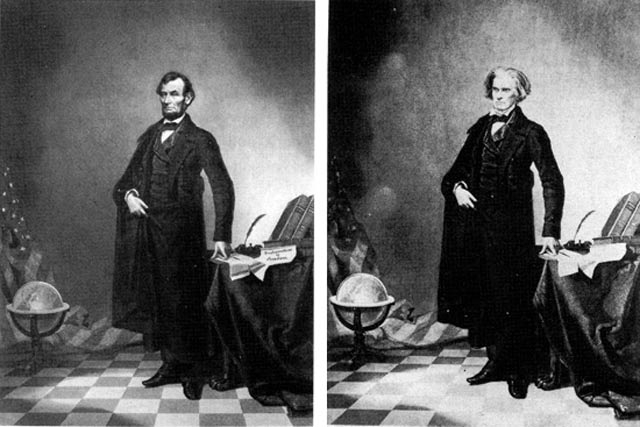
\includegraphics[width=\textwidth]{dissertation//figures/lincoln1960.jpg}
            \caption{A spliced portrait of Abraham Lincoln (left) with the original (right)\cite{singh2018art}}
            \label{fig:lincoln}
    \end{subfigure}
    \begin{subfigure}{0.45\textwidth}
        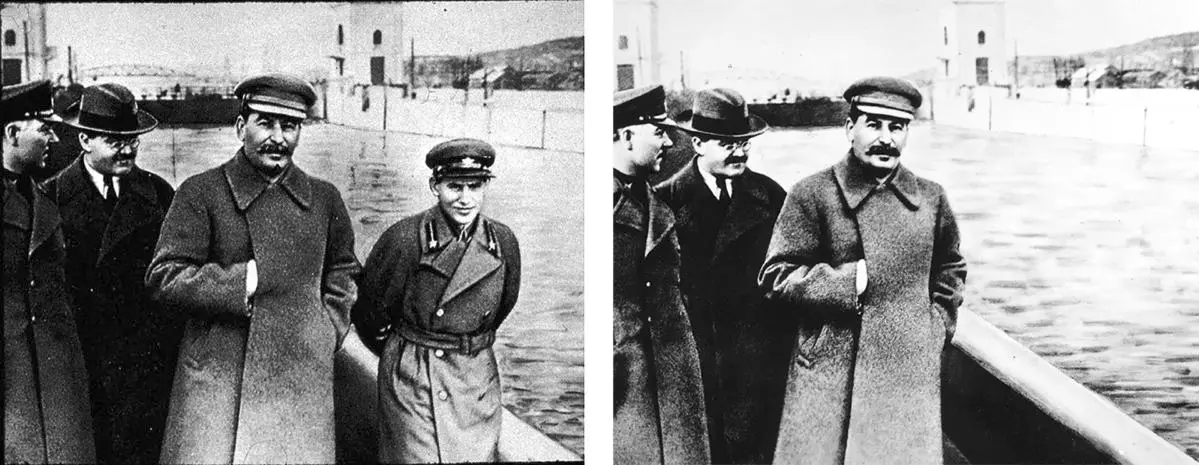
\includegraphics[width=\textwidth]{dissertation//figures/stalin.png}
        \caption{A photo of Stalin and Yezhov (left) which was subsequently edited to remove Yezhov (right)}
        \label{fig:stalin-yezhov}
    \end{subfigure}
    \caption{Examples of historical images that were edited}
    \label{fig:edited-images}
\end{figure}

With the advent of digital photography and computers, it photo manipulation became mainstream. Suddenly, images were not physical items but data stored on a computer which could be easily manipulated. Changes could be viewed instantly, reversed, and shared easily. Programs to edit images soon became possible such as Adobe Photoshop\footnote{\url{https://www.adobe.com/uk/products/photoshop.html}} and GIMP\footnote{\url{https://www.gimp.org/}}. Whilst these tools made photo editing cheap and accessible, they still required time, effort, and skill from humans in order to produce; an original image is also required for manipulation.

Computer Generated Imagery (CGI) is a technique primarily used in movies to add artificially augment a frame, often with complete novel additions. CGI was first used in the 1958 film ``Vertigo" and became widespread in the 1990s\cite{ozturk2023vicious}. In the present day, CGI is used in almost every blockbuster film to generate realistic images. In ``Rogue One: A Star Wars Story" the actor Peter Cushing digitally recreated after his death in 1994 to play Grand Moff Tarkin (Figure \ref{fig:tarkin}).While CGI requires large amounts of hardware, consumer image generation runs on much worse hardware but has equally progressed. Most modern social media apps contain a variety of beauty filters\cite{corcoran2014digital}. For example, a blur can be applied to reduce skin blemishes as shown by Figure \ref{fig:beauty-filter}. These are often less computationally expensive and so can run on smartphones, offering the ability to manipulate media to the masses, not just the technically-able and skilled.

\begin{figure}[h]
    \centering
    \begin{subfigure}{0.45\textwidth}
        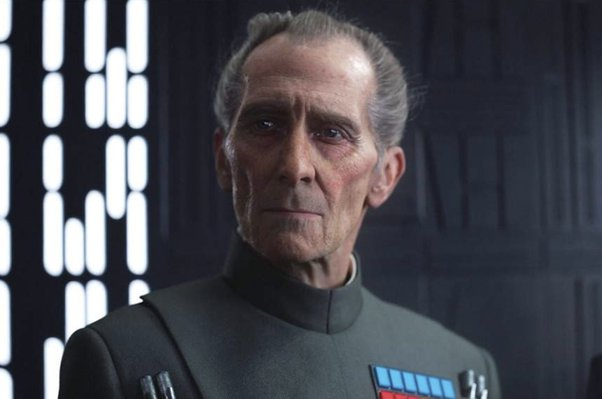
\includegraphics[width=\linewidth]{dissertation//figures/grandmoff-tarkin.jpg}
        \caption{A digital recreation of Peter Cushing for the film ``Rogue One: A Star Wars Story"\cite{rogueone}}
        \label{fig:tarkin}
    \end{subfigure}
    \begin{subfigure}{0.45\textwidth}
        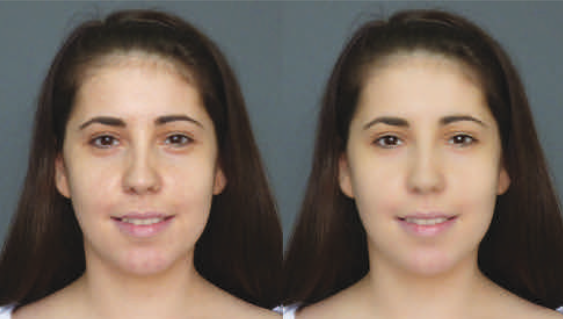
\includegraphics[width=\linewidth]{dissertation//figures/blurring.png}
        \caption{An original image (left) blurred to remove skin blemishes (right)\cite{corcoran2014digital}}
        \label{fig:beauty-filter}
    \end{subfigure}
    \caption{Examples of digital image manipulation}
    \label{fig:digital-manipulation}
\end{figure}

\subsection{Artificial Intelligence for Manipulating Media}

\subsubsection{Neural Networks}

DeepFakes are a type of AI known as neural networks. As described in Section \ref{sec:project-review}, neural networks are a subsection of AI designed of the structure of the human brain\cite{islam2019overview}. Traditional computation manipulates binary, whereas neural networks manipulate the connections between computational elements. Work on simulating the brain using mathematical functions began in 1920\cite{brush1967history}, 37 years before the academic formalisation of AI in 1957 at the Dartmouth Workshop\cite{crevier1993ai}. The field would remain relatively stagnant until the proposal of the Multi-Layer Perceptron (MLP) in 1958\cite{rosenblatt1958perceptron} and how it could ``learn" in 1967\cite{ivakhnenko1967cybernetics}.

Neural networks contain a collection of neurons organised into layers, each layer receives inputs from the neurons before (Figure \ref{fig:full-neural-network}). Each of the $n$ inputs has an associated weight ($w_i$) and value ($x_i$). Once the combined weights and an additional bias weight ($b$) exceed a determined threshold (usually 0) then the neuron fires with an output ($y$) determined by an activation function ($f(x)$). This is shown in Equation \ref{eq:neuron-activation} and Figure \ref{fig:neural-network}. The network shown in Figure \ref{fig:neural-network} has a 1 dimensional input, however MLPs can expand to an infinite number of dimensions.

\begin{equation}
\label{eq:neuron-activation}
    \begin{array}{c@{\hspace{2cm}}c}
        W = b+\displaystyle\sum_{i=1}^{n} w_ix_i  &
        y = \begin{cases}
            f(W) & \text{if } W \geq 0  \\
            0/-1 & \text{otherwise}
        \end{cases}
    \end{array}
\end{equation}

\begin{figure}[h]
    \centering
    \begin{subfigure}{0.45\textwidth}
        \centering
        \begin{tikzpicture}
            % inputs
            \node[draw=none] (x1) at (-1,2) {\(x_1\)};
            \node[draw=none] (x2) at (-1,0) {\(x_2\)};
            \node[draw=none] (x3) at (-1,-2) {\(x_3\)};
            
            % nuron (split circle)
            \node[draw, circle, minimum size=1.8cm, thick] (neuron) at (3,0) {};
            \node at (2.5, 0) {\(\sum\)}; % Left side - Summation
            \node at (3.5, 0) {\(f\)}; % Right side - Activation
            \draw[thick] (neuron.south) -- (neuron.north); % dividing line
            
            % output
            \node[draw=none] (output) at (6,0) {\(y\)};
            \draw[->] (neuron.east) -- (output);
            
            % weights
            \draw[->] (x1) -- node[above] {\(w_1\)} (neuron.west);
            \draw[->] (x2) -- node[above] {\(w_2\)} (neuron.west);
            \draw[->] (x3) -- node[below] {\(w_3\)} (neuron.west);
            
            % bias
            \node[draw=none] (bias) at (3,-2.5) {\(b\)};
            \draw[->] (bias) -- (neuron.south);
        \end{tikzpicture}
        \caption{Structure of a single artificial neuron}
        \label{fig:neuron}
    \end{subfigure}
    \begin{subfigure}{0.45\textwidth}
        \centering
        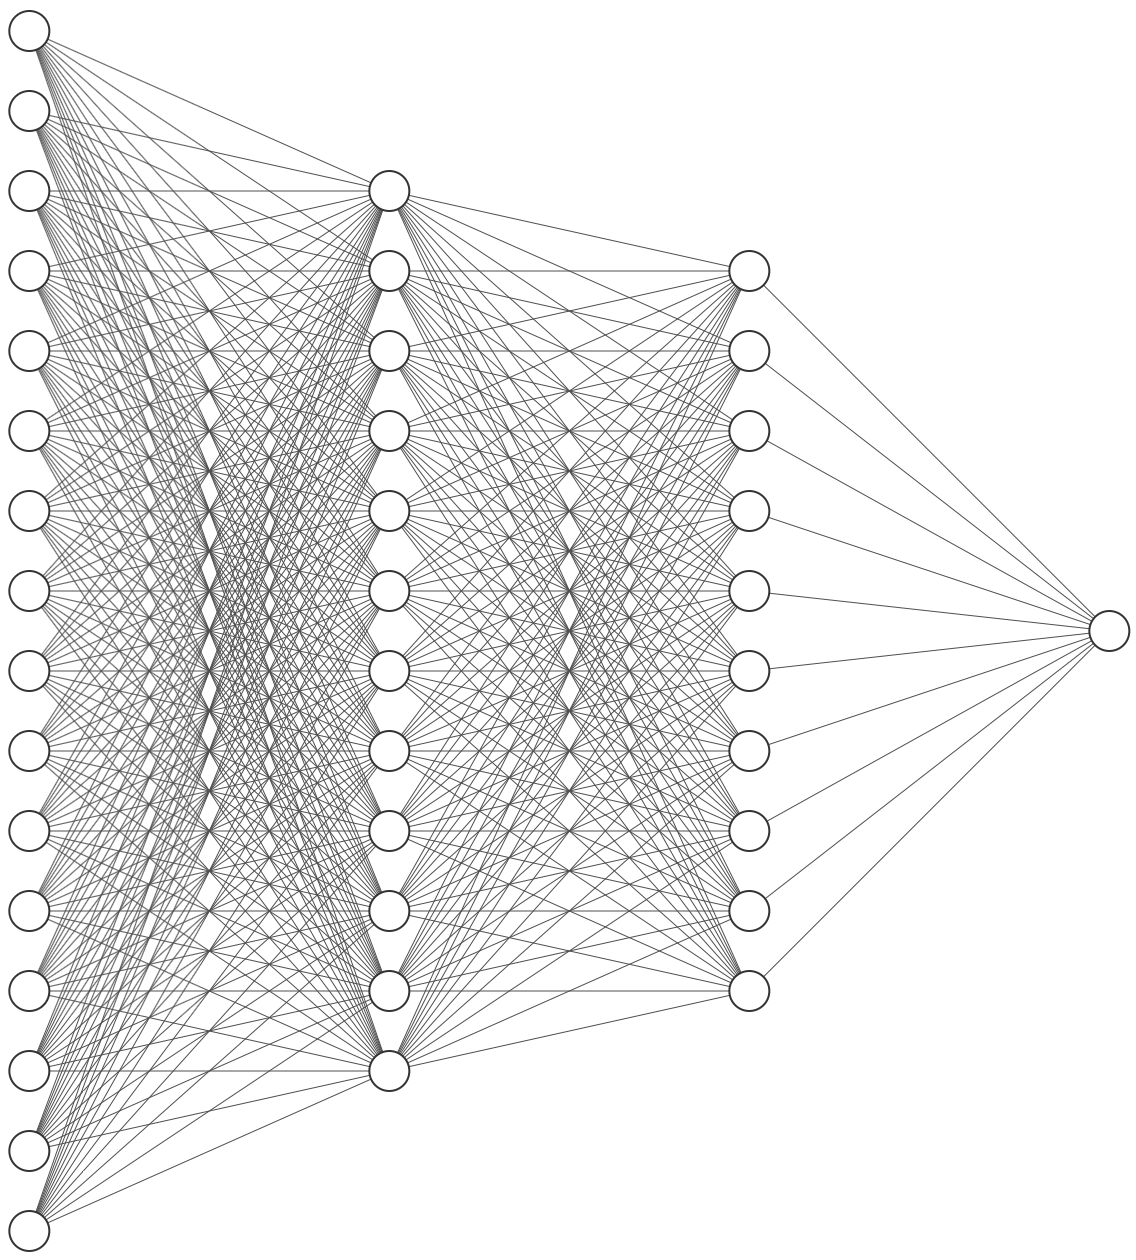
\includegraphics[width=0.75\textwidth]{dissertation//figures/generic-neural-diagram.png}
        \caption{A network of neurons split into layers}
        \label{fig:full-neural-network}
    \end{subfigure}
    \caption{A structure of a neural network and the individual neurons within it}
    \label{fig:neural-network}
\end{figure}

\subsubsection{Convolutional Neural Networks}
\label{sec:cnns}

Whilst MLPs are exceptionally powerful they can suffer from overfitting. Overfitting is where a machine learning model learns the training data, becoming exceptionally accurate in the training data but underperforms on any test data. With every neuron in an MLP layer being connected to all the neurons in the layers ahead and behind it, the network is prone to overfit\cite{o2015introduction}. A variety of methods can be employed to reduce overfitting, but the most common way removes connections from the network by reshaping the layers, this also has the attractive benefit of quicker computations as there are less weights to sum resulting in faster training and inference times. A number of methods to reduce connections have been proposed but the most successful are Convolutional Neural Networks (CNNs).

A CNN is a sequence of three layers: convolution layers, pooling layers, and a fully connected layer\cite{ibmconvolutional}. Each set of layers reduces the dimensions of the input, allowing each subsequent layer to take into account a larger portion of the image.

\begin{itemize}
    \item \textbf{Convolutional Layer}\\
    A Convolutional Layer is what a CNN lends its name to. It has two stages. The first stage is a filtering stage where a kernel (matrix) is passed over the input. The kernel is placed over the input and the dot product between the values in the kernel and the values in the input are calculated. This then becomes the output. The kernel is then shifted over by a fixed stride value to analyse another set of the input. This process is shown in Figure \ref{fig:filter}. The values (or weights) of each filter remain constant as it moves across the image, there can also be many filters, increasing the dimension of an input. These values are what are learned by this layer, by reducing the values to be trained to the size of the filter, this significantly speeds up the training process. Often some form of activation layer will be included to process the output array, more often than not, this uses the Rectified Linear Unit (ReLU) function, to limit outputs to strictly positive in order to introduce linerarity and prevent the vanishing gradient problem (a hindrance to learning)\cite{ibmconvolutional}.
    \begin{figure}[h]
        \centering
        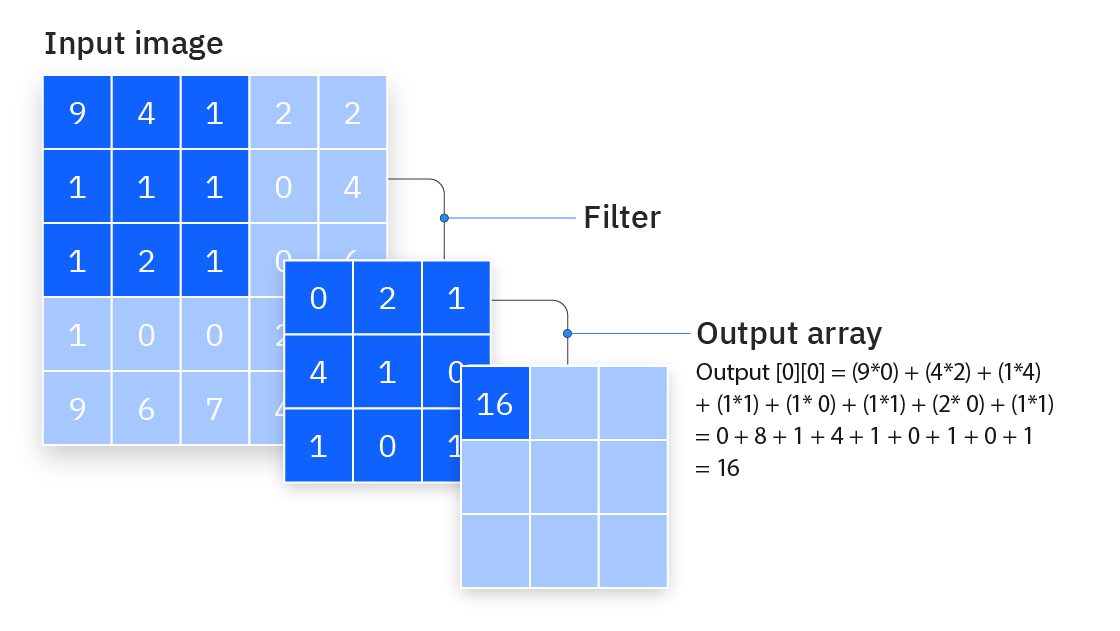
\includegraphics[width=0.5\linewidth]{dissertation//figures/cnn-filter.png}
        \caption{A diagram showing the action of a $3 \times 3$ filter\cite{ibmconvolutional}}
        \label{fig:filter}
    \end{figure}

    \item \textbf{Pooling Layer}\\
    The Pooling Layer is similar downsampling layer to the convolution layer but with no learnable parameters. Instead of a weighted kernel an aggregation function pools multiple values into a single one\cite{o2015introduction}. Any function could be used but the most common ones are: max pooling where the maximum value under the kernel is selected; or average pooling where the average of all the values is chosen. Pooling layers further reduce the numbers of learning parameters: reducing the tendency for overfitting, the model complexity, and computation time\cite{ibmconvolutional}.

    \item \textbf{Dense Layer}\\
    To produce an output that is usable a final dense layer is needed to convert the output of the previous layers into a desired shape. This is an fully connected MLP network.
\end{itemize}

A sequence of these layers are then combined to produce a network. The exact sequence and order is defined by the network architect and depends on the level of quality of output they want. More layers means a higher probable accuracy but incurs increased computation and tendency overfit. Further techniques exist to enhance CNNs such as skip connections which results in the outputs of layers to ``skip" forward layers and act as the input for layers further down the network. An example of a CNN to classify images is shown in Figure \ref{fig:sample-cnn}:

\begin{figure}[h]
    \centering
    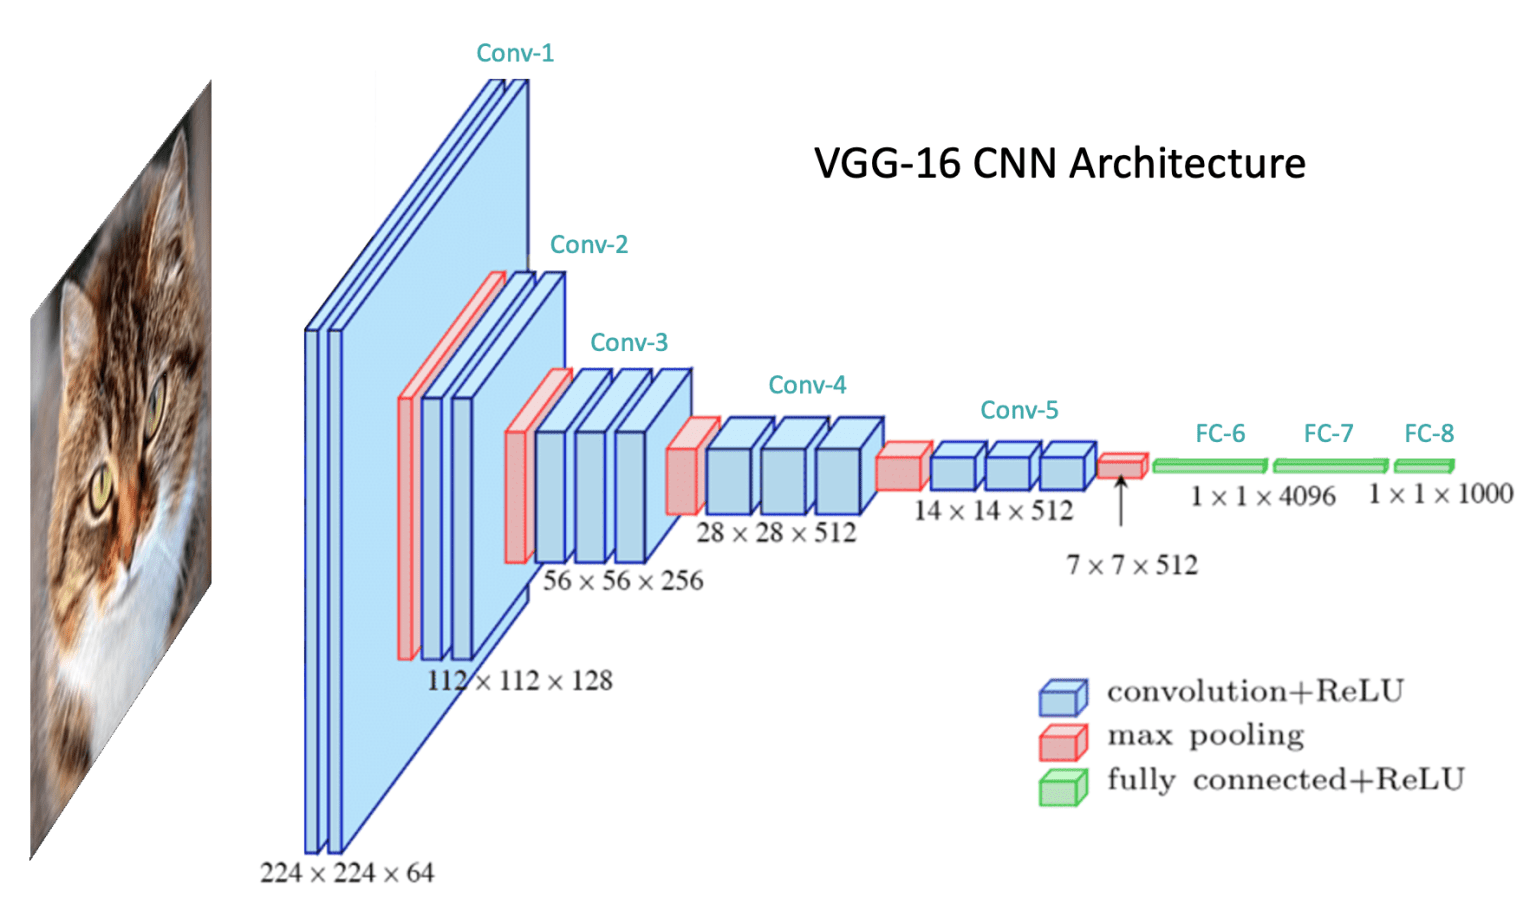
\includegraphics[width=0.5\linewidth]{dissertation//figures/sample-cnn.png}
    \caption{A sample convolutional neural network\cite{kromydas2023convolutional}}
    \label{fig:sample-cnn}
\end{figure}

\subsubsection{Learning}

The process of learning is similar across any kind of neural network. Every network will have trainable parameters (the kernel in a convolutional layer or the weights and biases in an MLP), these will be initialised randomly as hyperparameters. All learnable parameters are then trained in CNNs via a method called backward propagation of error (commonly shorted to backpropagation)\cite{rojas2013neural}.

This method of training requires a train set: a set of inputs and correct outputs. The backpropagation algorithm proceeds as follows:

\begin{enumerate}
    \item Each input is passed through the network in the forward pass. This produces one or more outputs
    \item The outputs are compared to the known truth outputs. A user-defined loss function evaluates how ``correct" the network's prediction is. The output of the loss function is a single value. Common loss functions are categorical cross entropy for classification tasks and Mean Squared Error (MSE) for location problems\cite{begmann-backpropagation}
    \item A backwards pass is then performed to differentiate the loss function and determine how much each learnable parameter contributes to the overall error. Every parameter $x$ in the network is connected to the output by a function $f(x)$, a composite function containing all of the activation functions and weights that combine with $x$ to reach the final output. By computing the partial derivative with respect to the loss function ($\frac{\partial L}{\partial x}$ where $L$ is the loss function), you can ascertain what the gradient for that particular value of parameter.
\end{enumerate}

For every parameter, the gradients over a set of inputs would like Figure \ref{fig:loss-graph} which indicated how much each parameter influences the final loss function. By minimising this graph, the loss function is minimised, resulting in an overall improvement to the network. Note the graph will often be a lot more complex compromising of a variety of hills, valleys, and plateaus.

\begin{figure}[h]
    \centering
    \begin{tikzpicture}
        % graph axis
        \draw[->] (0,0)--(3,0) node[midway,below]{$x$};
        \draw[->] (0,0)--(0,3) node[midway,left]{loss};
        %line
        \draw[domain=0.1:2.9] plot(\x,{(\x-1.5)^2+0.5});
    \end{tikzpicture}
    \caption{A sample plot of the value of the loss function over varying values of a parameter $x$}
    \label{fig:loss-graph}
\end{figure}

A variety of methods exist to find the minimum of the graph in the least possible steps. The most commonly used is Stochastic Gradient Descent (SGD)\cite{robbins1951stochastic}, first applied to neural networks in 1967\cite{shunichi1967theory}. SGD follows the following formula:

\begin{equation}
    x_n=x_{n-1}-\alpha l(x)
\end{equation}

$x_n$ is the new value of the parameter $x$ which has previous value $x_{n-1}$. This value is altered by $l(x)$, the gradient produced for that parameter by backpropagation. $\alpha$ is a hyperparameter representing the learning rate. Often a number close to 0, this limits how much the value can vary within the graph. Too low of learning rate results in slow learning and the potential to get stuck in local minima or plateaus. A high learning rate leads to the possibility of divergence and the minimum never being found.


\begin{figure}[h]
    \centering
    \begin{subfigure}{0.3\textwidth}
        \centering
        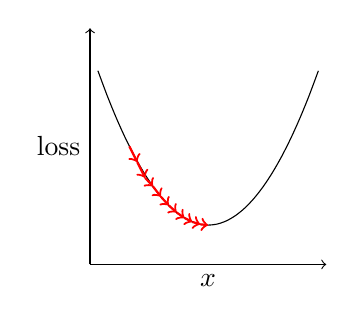
\begin{tikzpicture}
            % graph axis
            \draw[->] (0,0)--(3,0) node[midway,below]{$x$};
            \draw[->] (0,0)--(0,3) node[midway,left]{loss};
            % loss curve
            \draw[domain=0.1:2.9,smooth] plot(\x,{(\x-1.5)^2+0.5});
            % small steps
            \draw[->,red,thick] (0.5,1.5) -- (0.6,1.3);
            \draw[->,red,thick] (0.6,1.3) -- (0.7,1.1);
            \draw[->,red,thick] (0.7,1.1) -- (0.8,0.99);
            \draw[->,red,thick] (0.8,0.99) -- (0.9,0.86);
            \draw[->,red,thick] (0.9,0.86) -- (1.0,0.75);
            \draw[->,red,thick] (1.0,0.75) -- (1.1,0.66);
            \draw[->,red,thick] (1.1,0.66) -- (1.2,0.59);
            \draw[->,red,thick] (1.2,0.59) -- (1.3,0.54);
            \draw[->,red,thick] (1.3,0.54) -- (1.4,0.51);
            \draw[->,red,thick] (1.4,0.51) -- (1.5,0.5);
        \end{tikzpicture}
        \caption{Too low learning rate}
    \end{subfigure}
    \hfill
    \begin{subfigure}{0.3\textwidth}
        \centering
        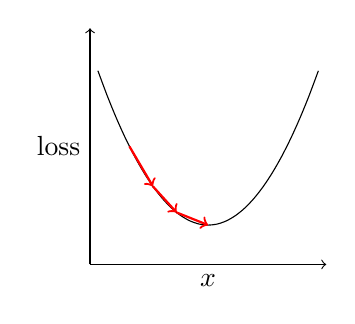
\begin{tikzpicture}
            % graph axis
            \draw[->] (0,0)--(3,0) node[midway,below]{$x$};
            \draw[->] (0,0)--(0,3) node[midway,left]{loss};
            % loss curve
            \draw[domain=0.1:2.9,smooth] plot(\x,{(\x-1.5)^2+0.5});
            % optimal steps
            \draw[->,red,thick] (0.5,1.5) -- (0.8,0.99);
            \draw[->,red,thick] (0.8,0.99) -- (1.1,0.66);
            \draw[->,red,thick] (1.1,0.66) -- (1.5,0.5);
        \end{tikzpicture}
        \caption{Optimal learning rate}
    \end{subfigure}
    \hfill
    \begin{subfigure}{0.3\textwidth}
        \centering
        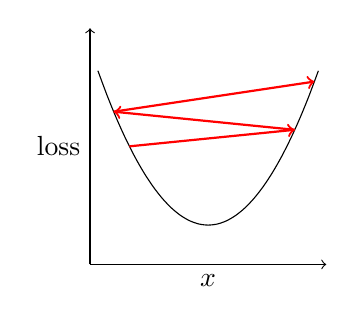
\begin{tikzpicture}
            % graph axis
            \draw[->] (0,0)--(3,0) node[midway,below]{$x$};
            \draw[->] (0,0)--(0,3) node[midway,left]{loss};
            % loss curve
            \draw[domain=0.1:2.9,smooth] plot(\x,{(\x-1.5)^2+0.5});
            % large steps
            \draw[->,red,thick] (0.5,1.5) -- (2.6,1.71);
            \draw[->,red,thick] (2.6,1.71) -- (0.3,1.94);
            \draw[->,red,thick] (0.3,1.94) -- (2.85,2.3225);
        \end{tikzpicture}
        \caption{Too high learning rate}
    \end{subfigure}
    \caption{Effect of different learning rates on loss function optimisation}
    \label{fig:learning-rates}
\end{figure}

Traditionally, finding an optimal learning rate has been a hard problem and thus a variety of methods have been introduced to give a larger safety net when choosing parameters. The most popular of these is the Adaptive Moment Estimator (commonly shortened to Adam)\cite{kingma2014adam}.

Adam combines the ideas of adaptive learning rate, and momentum. A per-parameter learning rate was first proposed in AdaGrad\cite{duchi2011adaptive} which implements a greater learning rate for sparser parameters (when the majority of weights are near zero) and lesser rates for denser parameters. Momentum fine tunes the learning rate for each parameter by combining it with the magnitude of the previous gradients.

When training, the above process will be done for every learnable parameter for every item in the trainset. Often the trainset will be too small to allow for meaningful learning. To combat this the dataset will be iterated over multiple times. One iteration over the entire dataset is referred to as an epoch\cite{begmann-backpropagation}. Often training will be done for a set number of epochs or until the loss function stabilises. 

\subsubsection{Generative Artificial Intelligence}

Whilst editing an image was easy, adding original content to an image was more difficult, requiring specialist expertise. The difficulty is further increased when trying to edit a video as more images need to be edited and be stitched seamlessly together. Generative AI (GenAI) is a form of neural network that can generate content. In images, they can adapt large amount of images to fit a specific goal or, in more recent works, convert written prompts into completely original images and videos.

The first notable GenAI was Generative Adversarial Networks (GANs)\cite{goodfellow2014generative}. GANs are two neural networks working together, a generator and a discriminator. The training process is ``a minimax two-player game": when one model looses by a certain amount, the other model gains an equal amount. In the context of image generation, the generator creates novel images based on a dataset from initial noise; the discriminator is fed a combination of the dataset and the generator's images, attempting to determine the origin of them. A diagram of a GAN network is shown in Figure \ref{fig:gan-diagram}. Over time, the generator becomes better and better at generating convincing images that fool the discriminator, eventually resulting in images that are nearly undetectable. The discriminator is a CNN, whereas the generator is a deconvolutional neural network\cite{zeiler2011adaptive}. Deconvolutional neural networks are CNNs but in reverse, where deconvolution layers convert a single value into an $n \times n$ square of new values.

\begin{figure}[h]
    \centering
    \begin{tikzpicture}[
        rect/.style={rectangle, draw=black, thick, minimum width=2.5cm, minimum height=1cm},
        bigrect/.style={rectangle, draw=black, thick, minimum width=6cm, minimum height=1cm}
    ]
        \node[rect] (nois) {noise};
        \node[rect] (gene) [above=of nois] {generator};
        \node[rect] (data) [above right=of nois] {dataset};
        \path (gene) -- (data) coordinate[midway] (midpoint);
        \coordinate (abovemid) at ($(midpoint) + (0,2cm)$);
        \node[bigrect] (disc) at (abovemid) {discriminator};

        \draw[->] (nois.north) -- (gene.south);
        \draw[->] (data.west) -- (gene.east);
        \draw[->] (gene.north) -- (disc.south -| gene.north);
        \draw[->] (data.north) -- (disc.south -| data.north);
    \end{tikzpicture}
    \caption{A diagram of the network structure of a Generative Adversarial Network}
    \label{fig:gan-diagram}
\end{figure}

Even in the original paper, GANs were being used to generate images of humans\cite{goodfellow2014generative}. In 2017, the technology would expand out of the realm of academia and into the public eye. A user named \verb|u/deepfakes| and others on the internet forum site Reddit\footnote{\url{https://reddit.com}} were discovered to be sharing pornographic material, edited to contain popular celebrities using GANs\cite{cole2018reddit}. Users were taking ``conventional" pornographic videos and using GANs to swap the faces to famous individuals without their consent. By only generating the face, these networks required less computational power and thus videos could be generated quickly. Following legal pressure, Reddit would delete the forum two months later\cite{cole2018reddit}, but the damage was done: it had been proven that AI could generate realistic videos of humans semi-autonomously. The media soon caught on to the story using the subreddit's name to coin the new types of videos as ``DeepFakes", a portmanteau of ``Deep Leaning" and ``fake".

Other methods of generating DeepFakes have been developed since GANs. Diffusion\cite{rombach2022high} is a process of removing noise from images based off of transformers\cite{vaswani2017attention}. When given random noise, these models can generate completely novel images. When trained on images with text descriptions, images could be generated from natural language prompts. Multiple different companies began making image generation tools such as OpenAI\cite{ramesh2022hierarchical}, Stable Diffusion\cite{stablediffusion2022}, and Midjourney\cite{midjourney2022}. OpenAI would go on to create Sora\cite{brooks2024video} a model that could generate realistic videos from a text prompt. The most recent architecture for image generators is Visual AutoRegressive modelling (VAR)\cite{tian2024visual}, also based on the transformer, that allowed image accuracy to scale with the amount of computational power available, enabling OpenAI to release 4o Image Generation\cite{4oimagegen}. Allowing for realistic images to be generated from a simple text prompt, such as Figure \ref{fig:gpt4o-dog}.

\begin{figure}[h]
    \centering
    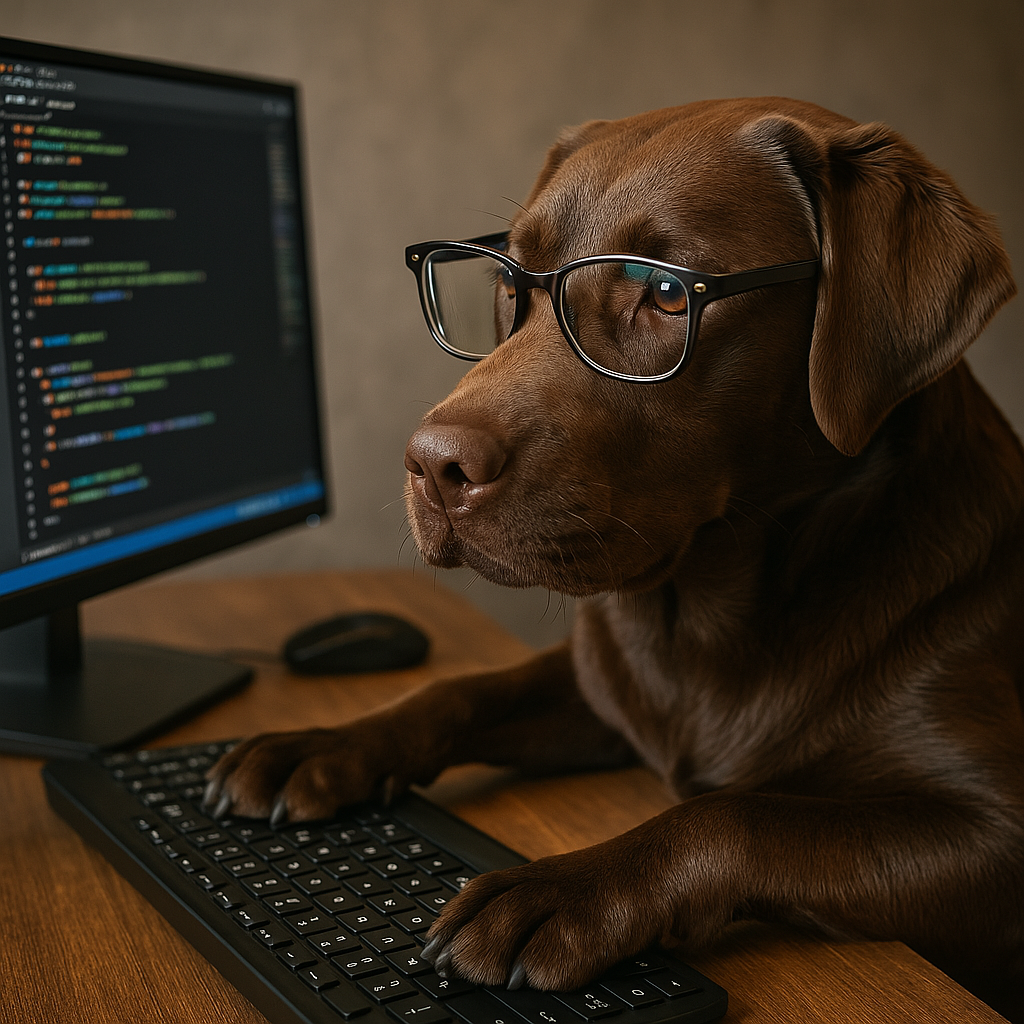
\includegraphics[width=0.5\linewidth]{dissertation//figures/gpt4o.png}
    \caption{An image generated by GPT-4o\cite{4oimagegen} using the prompt ``a chocolate labrador with glasses programming on a computer"}
    \label{fig:gpt4o-dog}
\end{figure}

\subsection{DeepFakes for Malicious Purposes}

DeepFakes can generate realistic images that are undetectable to humans. When presented with a combination of real and fake videos, individuals were asked to classify them as either real or DeepFaked; the overall accuracy was 55.54\%\cite{diel2024human}, only slightly better than guessing. Whilst DeepFakes rose to initial property for their entertainment value, for example users would use them to add the actor Nicholas Cage into movies he did not originally star in\cite{harris2023deep}. However, DeepFakes soon begun to be used for various malicious purposes.

DeepFakes have been used by state actors and opponents to misrepresent candidates in elections across the globe. In the United States 2016 election, Russian-backed faked videos were published on social media to ``undermine public faith in the U.S. democratic process, denigrate Secretary [Hilary] Clinton, and harm her electability and potential presidency"\cite{harris2023deep}. A similar misinformation campaign was attempted by Russia during the 2017 French elections where documents were stolen from Emmanuel Macron's campaign team and edited in an attempt to detriment his chances of being elected\cite{chesney2019deep}. They were unsuccessful with the Macaron team planting several fake documents which the Russians published along with poor coordination and obvious editing from the Russians. 

On an individual scale, DeepFakes have been used by scammers to fraud vulnerable people out of their money. A number of celebrities' likenesses have been used to promote products without their consent. Quantum AI is one such DeepFake-based scam\cite{sensity2024state}. DeepFakes videos of celebrities local to the area (such as Rishi Sunak or Justin Trudeau) were posted as social media advertisements endorsing the tool which guaranteed ``\$3,000 as early as day one". The second phase of the scam involved sockpuppets (non-existent people entirely AI generated) posing as local media reporting on the fake endorsements. Victims are prompted to invest a small amount of money to start with, often receiving genuine returns, soon however victims would be locked out of their account with their money stolen.

Another disturbing use for DeepFakes were around for their inception: pornography. Approximately 96\% of all DeepFakes generated are pornography\cite{ajder2019state}. Entire video sequences can be created from a handful of images scraped from an individual's public profiles\cite{chesney2019deep}. The videos generated are humiliating to the victims they depict, making them feel extremely vulnerable. Often these videos can then be used to further blackmail victims, threatening to release the videos publicly if the victim does not comply.

\section{DeepFake Detection}

With all the harm DeepFakes can do, it is essential to be able to detect them reliably and accurately. Early DeepFakes were easy to spot, often with warping around facial features and other temporal irregularities\cite{diel2024human}. Unfortunately, DeepFakes have become increasingly realistic and this trend is only set to continue. Taking inspiration from the GAN model (Figure \ref{fig:gan-diagram}), tools were developed to detect DeepFakes using AI. Whilst in the GAN architecture the generator is meant to win, discriminators are being generated with the aim to accurately detect DeepFakes. Significant investment and research is being made into DeepFake detection; the US government invested \$22,000,000 into DeepFake detection research with the Media and Semantic Forensics program\cite{harris2023deep}.

\subsection{Traditional Neural Network Detection Methods}

CNNs have been used to detect DeepFakes since the original GAN paper\cite{goodfellow2014generative}. Whilst CNNs are infinitely customisable with the different choices of layers and connections, often CNN architectures will consist of a backbone and a head\cite{elharrouss2024backbones}. Backbones are large convolutional neural networks that have been pre-trained on a large dataset that can extract features from an input. A customised head is then added to the network to convert the features into the desired output.

In context of DeepFake detection, the backbone is trained on ImageNet\cite{deng2009imagenet} an image dataset with 3.2 million images. Backbones are initially trained on the task of classifying an image in the dataset to an overall class (for example ``cat"). The backbone is then released with the weights from the training. For DeepFake detection, the head ends with a fully connected layer with a binary-softmax (Equation \ref{eq:softmax}) to classify an image into real or fake. Softmax separates $N$ input parameters into separate probabilities representing the probability that in input is in class $y$ such that $\sum^N_{i=1} y_i=1$. Using the initial weights of the backbone as the final weights of a similar problem is a technique known as transfer learning\cite{bozinovski1976influence} and can vastly improve the network's learning time and accuracy. The header's learnable parameters are initialised randomly as is normal. To extrapolate image classification to video classification, each frame of the video is independently classified and then the classifications are aggregated. Various aggregation methods exist but the simplest one is to set a threshold of frames that can be flagged as DeepFaked before the overall video is classified as fake.

\begin{equation}
    \label{eq:softmax}
    y_i=\frac{e^{z_i}}{e^{z_1} + e^{z_2}}, i\in1,2
\end{equation}

A variety of backbones have been applied to DeepFake detection to varying success\cite{thing2023deepfake}. The first backbones to be applied to DeepFake detection were VGG16/19\cite{simonyan2014very} and ResNet\cite{he2016deep}. Whilst VGG is a typical CNN as outlined in Section \ref{sec:cnns}, ResNet introduced the concept of skip-connections, allowing for the interaction of high and low level features. State of the art backbones have also been applied to DeepFakes, the best performing CNNs are currently EfficientNet\cite{tan2019efficientnet} and Xception\cite{chollet2017xception}. These achieve impressive accuracy on standard benchmarks (Section \ref{sec:datasets}), achieving over 90\%.

CNN detection works by pixel level analysis on the images. Due to the nature of CNNs it is difficult to tell what features they are focussing on for the final classification. However, due attention layers it is possible to view the regions of interest show in Figure \ref{fig:attention}, implying the particular areas of attention are the front facial features. Often these will be the area that DeepFakes will have the hardest time generating convincingly and will often leave artifacts such as inconsistent shaping\cite{verdoliva2020media}. CNNs are then picking up on these artifacts as features to classify a DeepFake. This leaves them vulnerable to possible pixel-based attacks which can disrupt the initial feature extraction\cite{gandhi2020adversarial}. Furthermore, reliance on specific artifacts cause CNNs to only be particularly effective on the DeepFake methodology they were trained and hence suffer reduced accuracy when viewing novel DeepFake methods\cite{thing2023deepfake}.

\begin{figure}[h]
    \centering
    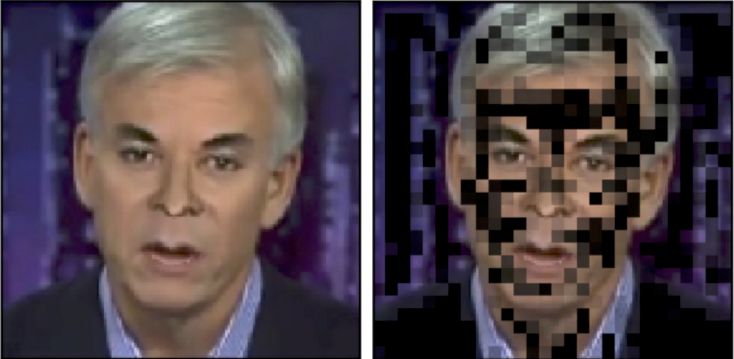
\includegraphics[width=0.5\linewidth]{dissertation//figures/attention-cnns.png}
    \caption{Output from attention layers of convolutional neural networks on DeepFake detection}
    \label{fig:attention}
\end{figure}

\subsection{Blink-Based Detection Methods}

% \begin{itemize}
%     \item Human's blink in a periodic and predictable manner
%     \item DeepFakes struggle with temporal stuff
%     \item Eye Aspect Ratio
%     \item DeepVision
%     \item Ictu Oculi
%     \item see progress report for evaluation and other stuff
% \end{itemize}

It has been shown that DeepFakes suffer from temporal inconsistencies\cite{juefei2022countering}. Temporal inconsistencies are where DeepFaked videos suffer from inconsistencies in between frames. For example, an object in the background may be temporarily obscured by the subject but when they move away from the object will have disappeared. 

A more subtle but ever present temporal inconsistency is blinking. Humans blink in a predictable manner, with the average person blinking for 0.1-0.4 seconds and a 2.8 second blink period\cite{schiffman1990sensation}. Timings can vary based on a number of factors like age, gender, time of day, and activity\cite{jung2020deepvision}; but, nevertheless, blinking remains a consistent physiological act that can be predicted but DeepFakes cannot reproduce.

\subsubsection{Eye Aspect Ratio}

To determine when an individual is blinking or not, the most common approach is the Eye Aspect Ratio (EAR)\cite{soukupova2016eye}. The EAR is a ratio of the distance between siz eye landmarks (Figure \ref{fig:ear}). 2 landmarks are labelled in caranucle and lateral canthus ($p_1$ and $p_4$, respectively) and the others are equidistant around the eyelid, labelled clockwise. The EAR is the ratio between the height and width of the eye (Equation \ref{eq:ear}) and is relatively constant when the eye is open but verges close to zero when closed. It is partially consistent between people and variations in poses. The modal person has two eyes and so the total EAR is taken as the average of the two eyes. When plotted as an EAR-time graph (Figure \ref{fig:ear-graph}), a blink is evident as a steep drop in the graph. 

\begin{figure}[h]
    \centering
    \begin{subfigure}{0.45\textwidth}
        \centering
        \begin{tikzpicture}
            \node[anchor=south west, inner sep=0] at (0,0) {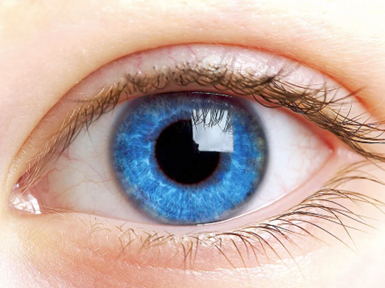
\includegraphics[width=\linewidth]{dissertation/figures/eye.png}};
            \filldraw[black] (0.7,1.7) circle (5pt) node[anchor=west, xshift=5pt] {$p_1$};
            \filldraw[black] (2.2,3.4) circle (5pt) node[anchor=north east, yshift=-5pt] {$p_2$};
            \filldraw[black] (4.6,3.5) circle (5pt) node[anchor=north west, xshift=3pt] {$p_3$};
            \filldraw[black] (6.2,2.6) circle (5pt) node[anchor=east, xshift=-5pt] {$p_4$};
            \filldraw[black] (4.5,1.4) circle (5pt) node[anchor=south west, xshift=4pt] {$p_5$};
            \filldraw[black] (2.8,1.2) circle (5pt) node[anchor=south east, xshift=-3pt] {$p_6$};
        \end{tikzpicture}
        \caption{An image of a human eye with the 6 points necessary for the Eye Aspect Ratio labelled}
        \label{fig:ear}
    \end{subfigure}
    \hfill
    \begin{subfigure}{0.45\textwidth}
        \centering
        \raisebox{1.8cm}{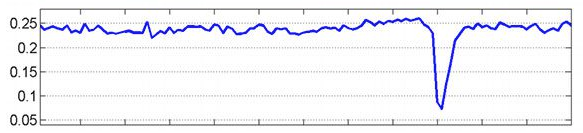
\includegraphics[width=\linewidth]{dissertation/figures/ear-graph.png}}
        \caption{A graph of EAR over time with a blink in the final third}
        \label{fig:ear-graph}
    \end{subfigure}
    \caption{The points and resulting graph for the Eye Aspect Ratio}
\end{figure}

\begin{equation}
    \label{eq:ear}
    EAR=\frac{||p_2-p_6|| + ||p_3-p_5||}{2||p_1-p_4||}
\end{equation}

\subsubsection{DeepVision}

DeepVision\cite{jung2020deepvision} is a detection model that utilises the $EAR$ and other environmental factors to determine whether a video is DeepFaked or not by comparing their blink patterns to a database of known ``good" blinking patterns.

DeepVision's input not only includes the video to be checked but a number of environmental factors. A user must manually estimate the: gender, age, time, and activity (whether the subject is moving or stationary) of the main subject of the video. 

Two algorithms are used to detect a blink. The first algorith is a target detector that uses Fast-HyperFace\cite{ranjan2017hyperface} which is a pretrained CNN that can identify subjects of a video and produce basic landmarks. If the detection confidence is over 70\%, the subject is identified as the target and a basic crop of their face is calculated from the landmarks and forwarded to the next algorithm.

A second algorithm takes the face crops and calculates $p_{1-6}$ for the $EAR$, whilst the exact algorithm is not defined, it is assumed to be the algorithm used in the original $EAR$ paper, Intraface\cite{xiong2013supervised}. From these six points, the $EAR$ is calculated for each eye and then averaged across the two. A blink is defined as when the $EAR$ drops below a certain threshold for multiple consecutive frames. DeepVision sets this threshold as two standard deviations below the mean. Data such as when the blink occurred in time, the period of blink, and frequency are then used as features for the next step.

DeepVision compares these features with known good features from a database. The database was created using known good data from the Eye Blinking Prediction Dataset\cite{turing2018eye}. The database is queried for individuals in the same environment as the subject and the corresponding features of blinking across the video are returned. The database's features are compared to the video's and if they are ``within an allowable" range the video is declared as real, otherwise fake. DeepVision achieves an overall accuracy of 87.5\%.

\begin{figure}[h]
    \centering
    \begin{subfigure}{0.45\textwidth}
        \centering
        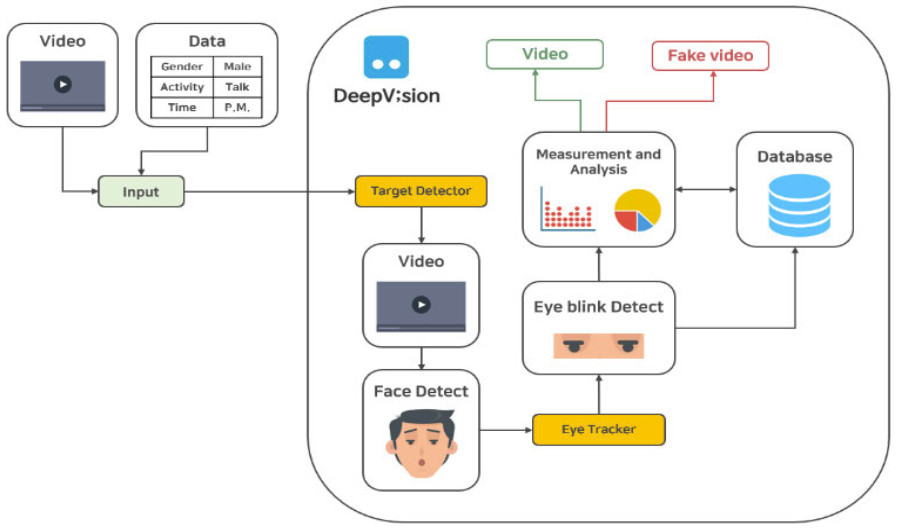
\includegraphics[width=\linewidth]{dissertation//figures/deepvision-flow.png}
        \caption{A flow diagram for DeepVision\cite{jung2020deepvision}}
        \label{fig:deepvision-flow}
    \end{subfigure}
    \hfill
    \begin{subfigure}{0.45\textwidth}
        \centering
        \raisebox{1.2cm}{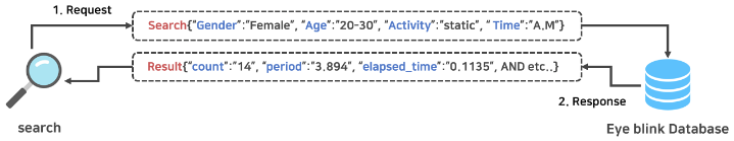
\includegraphics[width=\linewidth]{dissertation//figures/deepvision-database.png}}
        \caption{A sample database query for DeepVision\cite{jung2020deepvision}}
        \label{fig:deepvision-database}
    \end{subfigure}
    \caption{DeepVision's architecture and database queries}
    \label{fig:deepvision}
\end{figure}

DeepVision's primary advantage is that it is easy to compute and program. Fast-HyperFace is a pre-trained model and therefore is a simple drag-and-drop implementation. Once $p_{1-6}$ are located in a frame, it is a simple calculation to determine the EAR. The following statistical analysis to determine whether blinking is consistent with real videos is also relatively simple and non-computationally intensive as it is a database query. Therefore, any methodology involving DeepVision would be fast to implement and relatively easy to debug. It also benefits from more granularity in eye state data which could enable more complex analysis.

The primary downside to DeepVision is the potential occlusion of the eye(s). EAR requires the entire eye to be visible in the frame of a video to identify all of the points. A partial $EAR$ can be calculated with a single eye but the accuracy of this is going to be less than if two eyes were visible. The second disadvantage is the database required to determine whether blinking is consistent with normal blinking. The database requires many labelled examples which would be time-consuming to produce. Furthermore, the exact methodology for determining whether video's data is similar enough to the dataset's is never explained, nor is the ``allowable" range, resulting in DeepVision's accuracy being impossible to replicate

\subsubsection{Ictu Oculi}

Another method for blink-based DeepFake detection is Ictu Oculi\cite{li2018ictu}. A more complex method of blink-detection allows for a simpler method of blink verification. 

An initial pre-processing step is done to identify the faces of the image using dlib's\cite{king2009dlib} face detector and distort and crop them so that the face is: in the centre of the image; rotated such that the eyes form a horizontal line; and scaled to a similar size across the duration of the video. The main face is chosen as the one with the highest confidence. This face is further cropped to just the eyes which is then passed to the main model.

To determine the current state of the eye (open or closed), Ictu Oculi uses a custom Recurrent Neural Network (RNN). RNNs are a similar to CNNs but contain recurrent connections that can loop back into the network, allowing for a form of memory. This makes RNNs very effective for analysing time-based data as each position in time can be predicted using the context of the previous prediction; unlike, CNNs which would analyse each position independently.

The specific form of RNN used by Ictu Oculi is the Long Short-Term Memory (LSTM) modules\cite{hochreiter1997long}. LSTM modules dictate how many of the previous states to remember and how much influence the previous states have on the current state. Ictu Oculi consists of three main stages. The first stage is feature extraction using a VGG16-based CNN. Discriminative features are extracted from the cropped eye image. The features and the previous LSTM's output are fed into an LSTM in the sequence learning stage. This takes temporal features into account to enhance the blink detection; for example, if the previous five frames have all shown the eye in the process of closing, it is likely the current frame will also show the eye closing. The final stage is the state prediction which uses a dense MLP to determine whether the eye is open or closed. A full diagram is shown in Figure \ref{fig:ictu-oculi}.

\begin{figure}[h]
    \centering
    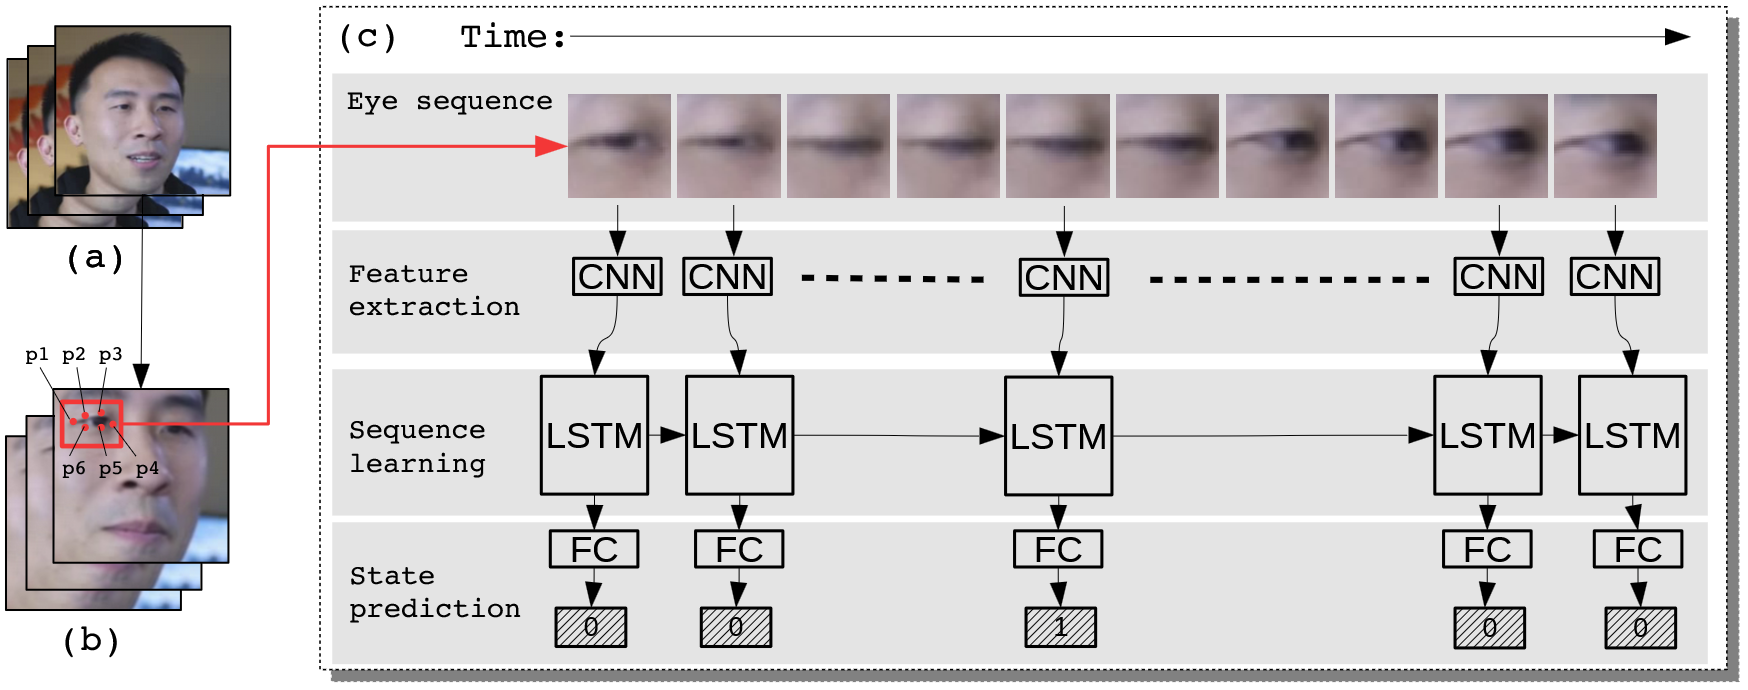
\includegraphics[width=0.75\linewidth]{dissertation//figures/ictu-oculi.png}
    \caption{A network diagram of Ictu Oculi\cite{li2018ictu}}
    \label{fig:ictu-oculi}
\end{figure}

As the accuracy of data is reduced from the amount an eye is open to a binary open/close, the simplicity of the validity algorithm needs to be greatly reduced. The algorithm implemented detects the number of blinks in a set period (60 seconds), the average person blinks 34.1 times a minute. A video is deemed fake or real based on how closely the blinking in the video matches this number. This leads to an accuracy of 99\% when tested on a custom dataset of 32 videos.

Ictu Oculi has a much more complex blink-detection system, requiring two separate machine learning models trained to identify if a blink is happening or not. This is more complex and requires pre-processing resulting in longer development and training times. On the other hand, it results in a much more resilient blink detection mechanism as the eye's state can be accurately determined even when partially obscured.

The drawback is that the state of the eye is binary open/close, any information relating to the speed of the blink is lost resulting in a very rudimentary system to determine whether a sequence of blinks is a DeepFake or not. Yet, this has little effect on the accuracy of detection.

\section{Adversarial Noise}

% \begin{itemize}
%     \item Additive noise can cause misclassification
%     \item Adversarial Perturbations
%     \item FakeRetouch
%     \item Again see progress report
% \end{itemize}

When operating on images, CNNs rely heavily on the individual pixels in the image. When these pixels are corrupted by noise it can seriously degrade the performance of CNNs\cite{yim2017enhancing}. For DeepFakes, this noise can cause a misclassification: a fake video could be classed as real and vice versa. Adversarial noise is deliberate noise added to an image to cause a desirable misclassification. Adversarial noise is aimed to be imperceptible to humans to avoid manual detection.

Malicious individuals can use noise to make their DeepFakes appear real by adding malicious noise to the final DeepFakes that will cause traditional CNNs to classify them as real. This becomes especially dangerous if a CNN is trusted to be accurate. Hypothetically, a CNN is produced that, on normal videos, is 100\% accurate and hence its classification is trusted absolutely. A malicious actor could add noise to their DeepFake, cause the CNN to declare it real, resulting in the DeepFaked video being trusted as real. Such a scenario is extremely dangerous and so it is important to develop noise resistant detection models.

There are a large number of methods that have been proven to cause misclassification of CNNs. A smaller subset of these have been proven effective on DeepFake classification. It is important to note that adversarial noise is only tested and applied to fake images.

\subsection{Fast Gradient Sign Method}
\label{sec:fgsm}

Fast Gradient Sign Method (FGSM)\cite{goodfellow2014explaining} is the simplest method for adding adversarial noise.

\begin{equation}
    \label{eq:fgsm}
    \mathbf{x}_{adv} = \mathbf{x} + \varepsilon \text{sign}(\nabla_x J(\mathbf{x},\mathbf{y}, \theta))
\end{equation}

$\mathbf{x}_{adv}$ and $\mathbf{x}$ are the perturbed and original frames, respectively. Note that the images are normalised such that $\mathbf{x}_{adv}\text{ and }\mathbf{x}\in[0,1]^3$. $J(\mathbf{x},\mathbf{y}, \theta)$ is the model's ($\theta$) training loss function on image $\textbf{x}$ and target class $\textbf{y}$. If the model's loss function is not known it must be guessed, however most classification models use some form of cross-entropy. Finally, $\epsilon$ is a hyperparameter to control the magnitude of noise. Higher values of $\epsilon$ add more noise to the image, increasing the chance of a misclassification from a CNN, but a similarly higher chance of being detected by humans.

The attack works by estimating the gradient of the loss function for the image $\textbf{x}$. By adding noise in the direction of that loss function, the model becomes less accurate, increasing the risk of misclassification. FGSM is simple and quick to compute as it only requires one call to the CNN being attacked. When tested against DeepFakes, FGSM reduced a ResNet-based detector from 95.4\% accuracy on fake images to 7.5\% accuracy\cite{gandhi2020adversarial}.

\subsection{Carlini-Wagner L2-Norm Attack}

A secondary adversarial noise shown to be effective on DeepFakes is the Carlini-Wagner L2-Norm (CW-L2) attack\cite{carlini2017towards}. It is more complex than FGSM and aims to minimise two objectives: reduce the L2-norm of the noise (Equation \ref{eq:cwl2-2}) whilst still adding enough noise to cause a misclassification (Equation \ref{eq:cwl2-3}).

\begin{align}
    \mathbf{x}_{adv} &= \frac{1}{2} \left( \tanh(\omega^*) + 1 \right) \label{eq:cwl2-1}\\
    \omega^* &= \arg\min_\omega \left( \|\mathbf{x'} - \mathbf{x}\|_2^2 + c f(\mathbf{x'}) \right) \label{eq:cwl2-2}\\
    f(\mathbf{x'}) &= \max\left( \max_{i \neq y} \left( \mathbf{Z}(\mathbf{x'})_y - \mathbf{Z}(\mathbf{x'})_i \right), -\kappa \right) \label{eq:cwl2-3}
\end{align}

Equation \ref{eq:cwl2-3} aims to cause the model to misclassify an image. $\mathbf{Z}(\textbf{x})$ is the pre-softmax vector output of the neural network, otherwise known as the logits of a model. This allows the CW-L2 attack to analyse the features that a model is using for a prediction rather than the final prediction. $\textbf{x'}$ is a sample perturbated image, $y$ is the index of the target class, and $i$ is the current classification. $\kappa$ acts as a hyperparameter threshold defining the minimum difference between the logits. By minimising $f(\textbf{x'})$, the difference between the logits of the correct class and the target class are maximised, raising the chances of a misclassification.

By minimising the L2-norm of the difference between the original and noisy image in Equation \ref{eq:cwl2-2}, the final noise chosen is the one with the least amount of noise, reducing the chance of humans spotting the noise. $c$ is another hyperparameter which controls the relative strength of each objective. Finally, the noise is normalised to $[0,1]$ in Equation \ref{eq:cwl2-1}.

Often, $c$ is found by a binary search during run time to further minimise the amount of noise on a frame by frame basis. To find the argument minimum (Equation \ref{eq:cwl2-2}) stochastic gradient descent is used, often with one thousand iteration steps. Both of these result in the CW-L2 attack taking a long time to run in comparison to other methods.

When tested on the same ResNet detector as FGSM (Section \ref{sec:fgsm}), the CW-L2 attack reduced the accuracy on fake videos from 95.4\% to 0\% accurate. Furthermore, it is more resistant to various noise-reducing filters that may be employed as defence\cite{gandhi2020adversarial}.

\subsection{FakeRetouch}

FakeRetouch\cite{huang2020fakeretouch} is a novel approach to adversarial noise that uses offline-trained CNNs. Instead of targeting a specific model, FakeRetouch aims to reduce the fingerprints of GANs that can show up in the Fourier Transform of an image. As shown in Figure \ref{fig:fakeretouch}, GANs have a much more nosier Fourier transform which some CNNs can leverage as a potential DeepFake identifier. FakeRetouch attempts to normalise the Fourier transform by removing the noise.

\begin{figure}[h]
    \centering
    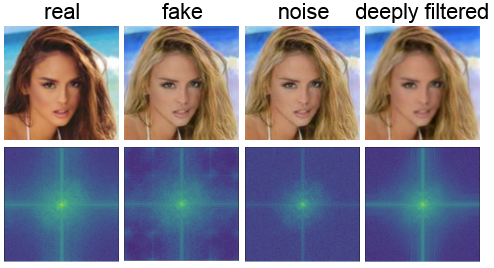
\includegraphics[width=0.5\linewidth]{dissertation//figures/fakeretouch-noise.png}
    \caption{A collection of images and their Fourier Transforms}
    \label{fig:fakeretouch}
\end{figure}

FakeRetouch is defined by the following equation:

\begin{align}
    \mathbf{x}_{adv} &= \mathbf{K} \circledast (\mathbf{x} + \mathbf{A}\odot \mathbf{N}_{\sigma}) \label{eq:fakeretouch-1}\\
    \text{Where } \mathbf{A} &= \arg \max_{\mathbf{A}} \left(J(\mathbf{x}+\mathbf{A},y,\theta)+||\mathbf{A}||_1\right) \label{eq:fakeretouch-2}
\end{align}

The offline trained CNN is a Kernel Prediction Network (KPN)\cite{mildenhall2018burst}. This produces a kernel, similar to the filters in a CNN, that averages out a certain area of pixels to reduce the noise in the image. This can be sufficient for conventional noise reduction but is unfortunately not successful to cause misclassification\cite{huang2020fakeretouch} so further noise is required.

FakeRetouch uses Gaussian Noise ($\textbf{N}_{\sigma}$ to further blur the image, to reduce the effect of the Gaussian noise it is passed through a binary map $\textbf{A}$, that only allows noise in certain areas of the image. It is desirable that $\textbf{A}$ is as sparse as possible to avoid human detection of the noise and hence $\textbf{A}$ is regulated by Equation \ref{eq:fakeretouch-2}. $J$ is the defined the same as Equation \ref{eq:fgsm} but is set as categorical cross-entropy. $y$ is the true class label of the image $\textbf{x}$. Equation \ref{eq:fakeretouch-2} regulates the amount of Gaussian noise added to a frame by minimising the L1-norm of the noise.

When tested on DeepFakes, FakeRetouch has limited success. It does not target the neural network directly and so relies on both the neural network analysing the Fourier transform of an image and the DeepFake generator producing excessive fingerprints in the Fourier space. For scenarios when both requirements hold, FakeRetouch reduces accuracy by 67\%; on the other hand, in scenarios where either one or none of the conditions hold, FakeRetouch either decreases detection by an insignificant amount or can even increase the accuracy of detection.

\section{Datasets}
\label{sec:datasets}

To compare performance of multiple proposed models, common datasets of DeepFakes were made. Datasets are large collections of data relevant to a problem that have been collated and labelled by a third party. For DeepFakes, these datasets take the form of videos or images that have been scraped from the internet. These are then passed into at least one DeepFake generator which produces a set of known fake media. This project is only concerned with videos.

FaceForensics++\cite{roessler2018faceforensics}\cite{roessler2019faceforensicspp} is one of the most popular datasets for DeepFake detection on videos. One thousand images were taken from YouTube and then were DeepFaked with four different methods: Fac2Face\cite{thies2016face2face}, FaceSwap\cite{kowalski2016faceswap}, DeepFakes\cite{deepfakes}, and NeuralTextures\cite{thies2019deferred}. This results in a total of four thousand videos to train data on. 

As part of a 2020 Kaggle competition, Meta released the DeepFake Detection Challenge (DFDC) dataset\cite{dolhansky2020deepfake}. Eight facial modification algorithms were used to create a unique dataset of approximately 124,000 videos. The DFDC is by far the most extensive dataset available. A further testest is also available for use that was not available to participants of the competition although this is not used when benchmarking.

Celebrities are often used in DeepFakes due to their popularity. A number of datasets based celebrities have been created, these are easier to create as videos involving celebrities are easier to license and larger in number than the typical individual. Celeb-DF\cite{li2020celeb} uses videos of 59 celebrities taken from YouTube. 590 real videos are altered using a custom algorithm to make 5,639 DeepFaked videos. Celebrities were specifically selected to cover a wide range of age, gender, race, and ethnicity. Another dataset that uses videos of celebrities is FakeAVCeleb\cite{khalid2021fakeavceleb}. As the name suggests, its an audio-visual model, able to fake both the sound and visual components of a video. Similar to CelebDF, videos were deliberatlry chosen to promote diversity within the dataset. Five hundred videos were altered using four algorithms to create 19,500 videos.